\documentclass{article}

\usepackage{repsty}

\newcommand{\uvec}[1]{\boldsymbol{\hat{#1}}}
\newcommand{\abs}[1]{\vert#1\vert}
\newcommand{\proj}[2]{\pi_{\uvec{#2}}\vec{#1}}

\newcommand{\Dw}{\Delta\omega}
\newcommand{\ii}{\imath}
\begin{document}

\section{Projection of polarization}
\begin{align}
	\vec{P} &= \sum_i \vec{s}, \notag\\
	\proj{s}{y} &\equiv \uvec{y}\cdot\vec{s} = \abs{\vec{s}}\cos\Theta, \notag\\
	\proj{P}{y} &= \sum_i \proj{s_i}{y} = \abs{\vec{s}}\sum_i \cos\Theta_i, \label{eq:SumSpins}\\
	\Theta_i &= \omega_i\cdot t + \phi_i,~ f(\phi_i),~g(\omega_i).\notag
\end{align}
$f$ and $g$ are distributions.

The phase $\Theta_i$ is a random variable, hence $\proj{P}{y}$ is a sum of random variables; this sum is distributed normally, with expectation $\Xpct{\proj{P}{y}}[t] = \abs{\vec{s}}\cdot n_b\cdot \int_\infty\cos\theta\cdot f(\theta|t)\td\theta$.

\section{Simulation}
\newcommand{\Norm}{\mathcal{N}}
\newcommand{\dy}{\Delta\gamma}
\newcommand{\ycoef}{h}
\newcommand{\wcoef}{G}
\newcommand{\dwcoef}{g}
In the simulation the following model was assumed:
\begin{align*}
	\dy &\sim \Norm(0, \SD{\dy}), \\
	\SD{\dy}(t) &= \SD{\dy}(0) + \ycoef\cdot t, \\
	\omega_i &= \omega_0 + \wcoef\cdot \dy_i^2, \\
	\phi &\sim \Norm(\phi_0, \SD{\phi}).
\end{align*}

\subsection{Constant $\SD{\dy}$}
When the beam particles' phase and oscillation frequency have unchanging distributions as in Figure~\ref{fig:PSdist_cDy}, the resulting polarization signal, computed according to eq.~\eqref{eq:SumSpins}, is shown in Figure~\ref{fig:Sgl_cDyPhys}.
\begin{figure}[h]
	\centering
	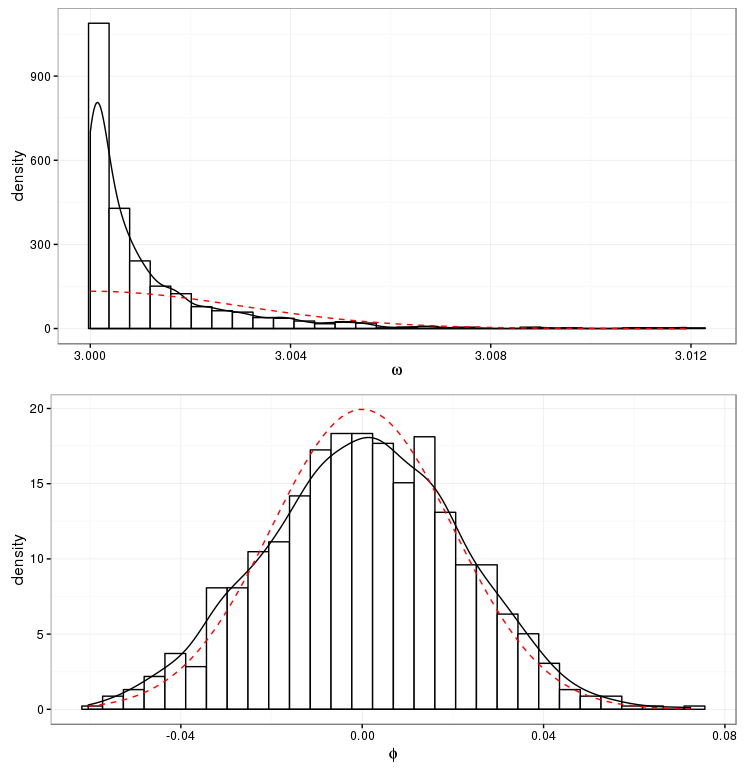
\includegraphics[scale=.5]{../img/PS_dist}
	\caption{Phase space distributions.\label{fig:PSdist_cDy}}
\end{figure}
\begin{figure}[h]
	\centering
	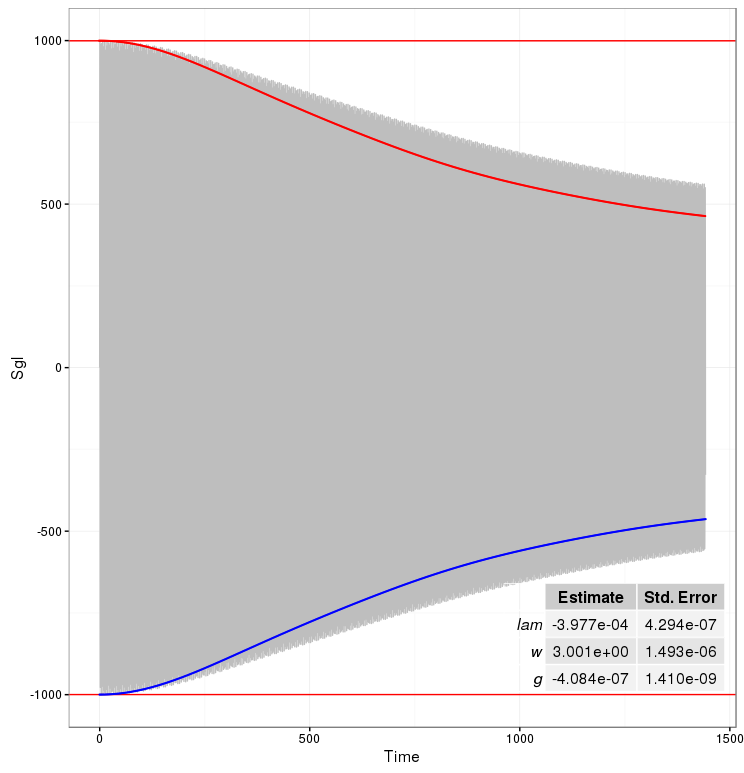
\includegraphics[scale=.6]{../img/Sgl_PhysDistros}
	\caption{Polarization signal in the case of constant phase space distributions. The read and blue lines mark are measurements taken at the points $\frac{2\pi n - \phi_0 +\pi/2}{\omega_0}$ and $\frac{2\pi n - \phi_0 +3\pi/2}{\omega_0}$ respectively.\label{fig:Sgl_cDyPhys}}
\end{figure}
\begin{figure}[h]
	\centering
	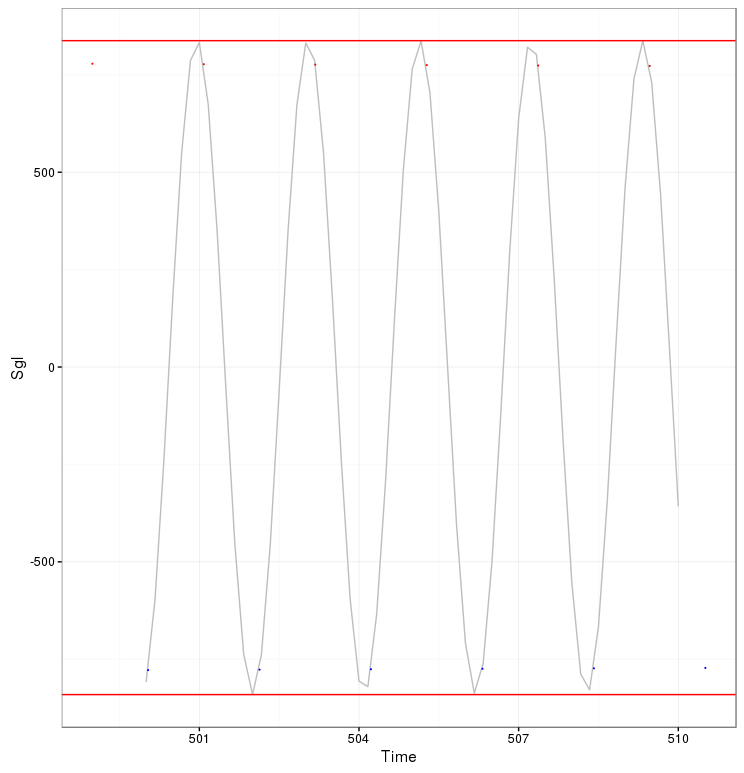
\includegraphics[scale=.5]{../img/Peaks_after_Peaks}
	\caption{Focus.\label{fig:Focus}}
\end{figure}

One can observe (Figure~\ref{fig:Focus}) that the read/blue lines, marking the measurements supposed to be at the peaks/valleys of the signal (null envelope), fall in front of the actual extrema after a while, which suggests that the signal's frequency is greater than that of the synchronous particle, $\omega_0$. With that in mind, we fitted the function $f(t) = n_b\cdot\exp\bkt{\lambda t}\cdot\sin\bkt{(\omega+\dwcoef\cdot t)\cdot t + \phi_0}$ to the simulated data.

The model fit yielded an $\hat{\omega} \approx 3.001 \pm 1.493\cdot10^{-6}$, and a life-time $\hat{\tau}\approx 2500$ sec. The frequency growth factor, $g$, is estimated $\dwcoef < 0$, indicating a \emph{decreasing} oscillation frequency. The estimate of $g$ is statistically significant, with the t-value $\approx 290$; we note, however, that the used model is drastically misspecified,~\footnote{The first derivative of the signal's envelope falls much slower at the beginning.} which might be the cause of the contradiction between the frequency's supposed deceleration, and the evidence of the computed envelope points. 

The signal's power spectrum (Figure~\ref{fig:PSD_cDyPhys}) mimics the particles' $\omega$ density distribution.
\begin{figure}[h]
	\centering
	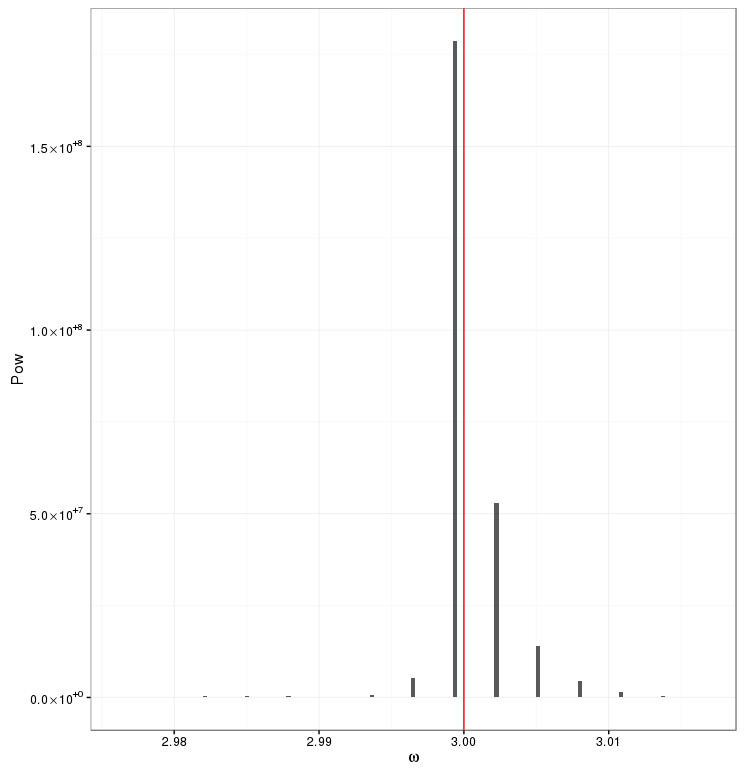
\includegraphics[scale=.5]{../img/Spec_PhysDistros}
	\caption{Power spectral density plot.\label{fig:PSD_cDyPhys}}
\end{figure}



\end{document}